\documentclass[
    11pt,
    a4paper,
    sfdefaults=false,
    toc=chapterentrywithdots,
    twoside,openright,
    titlepage,
    parskip=half,
    headings=normal,  % reduces heading size
    listof=totoc,
    bibliography=totoc,
    index=totoc,
    captions=tableheading,  % caption below table
    chapterprefix,
    listof=flat,
    final
]{scrbook}

% details about your thesis
\newcommand{\titel}{KOM-3 Objektserialisierung}
\newcommand{\artderarbeit}{Schriftliche Ausarbeitung}  % {Bachelorarbeit,Masterarbeit}
\newcommand{\autor}{Leon Breidt}
\newcommand{\studiengang}{Informatik}  % {Informatik,Wirtschaftsinformatik,Medieninformatik}
\newcommand{\matrikelnr}{377\,2588}
\newcommand{\erstgutachter}{Prof.\,Dr.~Ingo Scholz}
\newcommand{\zweitgutachter}{Prof.\,Dr.~Bartosz von\,Rymon\,Lipinski}
\newcommand{\betreuer}{M.Sc.\,~Martina Schmidt}
\newcommand{\unternehmen}{Musterfirma GmbH}
\newcommand{\logo}{figures/TH-Nuernberg-RGB.png}
\newcommand{\keywords}{hot, fuzz}
 

% custom head and foot
\usepackage[automark]{scrlayer-scrpage}
\pagestyle{scrheadings}
\ihead{\headmark}
\chead{}
\ohead{\pagemark}
\renewcommand*\chaptermarkformat{\chapappifchapterprefix{\ }% 
  \thechapter.\enskip}

\RedeclareSectionCommand[tocindent=0pt]{section}
\RedeclareSectionCommand[tocindent=0pt]{subsection}
%\RedeclareSectionCommand[tocnumwidth=70pt]{chapter}

%\usepackage{scrhack}

% other packages
\usepackage[utf8]{inputenc}
\usepackage[T1]{fontenc}
\usepackage{lmodern,relsize,textcomp,csquotes}
\usepackage{amsmath,amsfonts}
\usepackage[english,ngerman]{babel} 
\usepackage[final]{graphicx}
\usepackage{setspace,geometry,xcolor}
\usepackage{makeidx}
\usepackage{paralist,ifthen,todonotes}
\usepackage{url}
\usepackage[toc]{glossaries}
\usepackage{pdfpages}

% table setup
\usepackage{longtable}
\usepackage{array}
\usepackage{ragged2e}
\usepackage{lscape}

% pdf hyperref
\usepackage[
    bookmarks=true,
    bookmarksopen=true,
    bookmarksnumbered=true,
    bookmarksopenlevel=1,
    pdftitle={\titel},
    pdfauthor={\autor},
    pdfcreator={\autor},
    pdfsubject={\titel},
    pdfkeywords={\keywords},
    pdfpagelabels=true,
    colorlinks=true,
    linkcolor=red,
    urlcolor=magenta,
    anchorcolor=black,
    citecolor=cyan,
    filecolor=magenta,
    menucolor=red,
    plainpages=false,
    hypertexnames=true,
    linktocpage=true,
]{hyperref}

% configure your listings style
\usepackage{listings}
\lstset{
	tabsize=3,
	extendedchars=true,
	frame=single,
	showstringspaces=true,
	numbers=left,
	numberstyle=\small,
	breakautoindent=true
}

% page setup
% \setlength{\topskip}{\ht\strutbox}
\geometry{paper=a4paper,left=2.5cm,top=3.0cm,bindingoffset=.8cm}
\onehalfspacing
\frenchspacing
\clubpenalty = 10000
\widowpenalty = 10000 
\displaywidowpenalty = 10000

% some commands
\newcommand{\ua}{\mbox{u.\,a.\ }}
\newcommand{\zB}{\mbox{z.\,B.\ }}
\newcommand{\dahe}{\mbox{d.\,h.,\ }}
\newcommand{\bzw}{\mbox{bzw.\ }}
\newcommand{\bzgl}{\mbox{bzgl.\ }}
\newcommand{\eg}{\mbox{e.\,g.\ }}
\newcommand{\ie}{\mbox{i.\,e.\ }}
\newcommand{\wrt}{\mbox{w.\,r.\,t.\ }}
\newcommand{\etal}{\mbox{\emph{et.\,al.\ }}}


% TODO remove if not needed...
\usepackage{blindtext}

% load glossary entries
\makenoidxglossaries
\loadglsentries{glossary}

\begin{document}

\setcounter{secnumdepth}{3}  % numerate subsections
\setcounter{tocdepth}{2}  % ...but don't include them in toc

\frontmatter
\thispagestyle{empty}
\pdfbookmark[1]{Cover}{cov}
\begin{titlepage}

\begin{center}


\includegraphics[width=\linewidth]{figures/ohm-logo.png}\\[1cm]
\LARGE{Fakultät Informatik}\\[2cm]

\huge
\textbf{\titel}\\[1cm]
%
\Large
\artderarbeit~im Studiengang \studiengang\\[1cm]
%
\large
vorgelegt von

\Large
\autor\\[0.5cm]
\small
Matrikelnummer \matrikelnr\\[2cm]

\vspace*{\fill}

\large
\begin{tabular}{p{3cm}p{8cm}}\\
Betreuer:  & \quad \erstgutachter\\[1.2ex]
%Zweitgutachter: & \quad \zweitgutachter\\[1.2ex]
%discomment "Betreuer" and "Unternehmen" for a thesis in a company
%Betreuer: & \quad \betreuer\\
%Unternehmen: & \quad \unternehmen
\end{tabular}
\end{center}

\begin{center}
\copyright\,\the\year
\end{center}

\vspace{-0.5cm}
\singlespacing
\small
\noindent Dieses Werk einschließlich seiner Teile ist \textbf{urheberrechtlich geschützt}.
Jede Verwertung außerhalb der engen Grenzen des Urheberrechtsgesetzes ist ohne Zustimmung des Autors unzulässig und strafbar.
Das gilt insbesondere für Vervielfältigungen, Übersetzungen, Mikroverfilmungen sowie die Einspeicherung und Verarbeitung in elektronischen Systemen.

\end{titlepage}
\cleardoublepage

% download the following form and complete it (hit save in your editor)
% https://intern.ohmportal.de/fileadmin/Gelenkte_Doks/Abt/SZS/SB/SB_0050_FO_Pruefungsrechtliche_Erklaerung_und_Erklaerung_zur_Veroeffentlichung_der_Abschlussarbeit_public.pdf
%\includepdf{SB_0050_FO_Pruefungsrechtliche_Erklaerung_und_Erklaerung_zur_Veroeffentlichung_der_Abschlussarbeit_public.pdf}\cleardoublepage

\thispagestyle{empty}
\section*{Kurzdarstellung}
\label{sec:kurzdarstellung}
    
In dieser Ausarbeitung werden die Konzepte und Methoden der Objektserialisierung untersucht. Diese sind für die Effizienz und Zuverlässigkeit bei der Entwicklung der festgelegten Spieleideen von entscheidender Bedeutung. Beginnend mit einer Definition der Objektserialisierung, werten verschiedene Verfahren und Techniken dargelegt. Der Umgang mit referenzierten Daten und die Implementierung von Kompressionsmethoden zur Optimierung der Datenübertragung werden ebenfalls erklärt.

Ein weiterer Teil der Arbeit ist der Vergleich zwischen klassischen, strukturierten Datenformaten wie JSON und XML und effizienteren, auf Leistung ausgerichteten Formaten wie Protobuf, Cap’n Proto und Flatbuffers. Diese Diskussion dient als Grundlage für die Entscheidung, welche Bibliotheken für die beiden Projekte Park Chase und Into The Sky verwendet werden

Abschließend wird die Umsetzung der gewählten Verfahren für die beiden Projekte beschrieben. Neben einer ersten Implementierung sind hierbei auch die Testfälle wichtig, mit der die Funktionalität der Implementierungen sichergestellt werden.

\cleardoublepage

\tableofcontents

\mainmatter

\chapter{Theoretische Grundlagen}
\section{Begriffsdefinition und Anwendung}

Der Begriff "Objektserialisierung" beschreibt in der Informatik den Prozess, der Datenstrukturen in eine Reihe an Bytes übersetzt. Dies ist nützlich, um Objekte in eine Datenbank oder in eine Datei zu persistieren. Außerdem können Objekte so über ein Netzwerk übertragen werden, was eine der Hauptanwendungen ist. \cite{SerialisationIntroduction}

Das Gegenstück, also Objekte aus einem Datenstrom wieder aufzubauen, nennt sich Deserialisierung.

\section{Verfahren zur Serialisierung}

Es gibt eine große Bandbreite an Verfahren zur Serialisierung. Die Herausforderung ist es, für die hier vorliegenden Projekte die optimale Wahl zu treffen. Eine solche Wahl muss mehrere Eigenschaften optimieren:

\begin{itemize}
	\item Bandbreiteneffizienz
	\item Speichereffizienz
	\item Geschwindigkeit des Serialisierungsprozesses
	\item Erweiterbarkeit
	\item Interoperabilität
\end{itemize}

Neben der Auswahl eines geeigneten Protokolls, kann auch die Anwendung zusätzlicher Techniken, wie Delta-Serialisierung, sinnvoll sein. Außerdem ist die Vorauswahl von Daten wichtig. Man muss sich also im Vorhinein Gedanken darüber machen, welche Daten überhaupt in welchen Intervallen übertragen werden müssen.

\section{Umgang mit referenzierten Daten}

Daten, die über ein Netzwerk empfangen werden, beziehen sich oft auf Daten, die bereits in der Vergangenheit übertragen wurden, oder die noch gesendet werden. Es gibt zwei Herangehensweisen, die unabhängig von der Serialisierungsart möglich sind: Einbettung von Datenstrukturen oder Referenzierung über eindeutige Kennzeichnungen.

Beim Einbetten von Datenstrukturen werden die zu referenzierenden Daten direkt mit übertragen. Das bedeutet, dass insgesamt möglichst alle relevanten Daten gemeinsam übertragen werden. Dies hat den Vorteil, dass keine dauerhafte Speicherung der übertragenden Daten nötig ist. Die Daten können direkt und vollständig als Block übertragen und verarbeitet werden. Der Nachteil ist, dass so automatisch größere Datenpakete übertragen werden müssen. Dies dauert also insgesamt länger und man muss mit der Verarbeitung warten, bis alle Daten übertragen sind.

Wenn die Daten untereinander referenziert werden, so geschieht dies durch einen eindeutigen Kennzeichner. Oft werden hierfür einfache Zahlenwerte benutzt, aber auch die Verwendung von UUIDs (Universally Unique Identifiers) ist sehr geläufig. Diese Werte sind entweder in ihrem Gültigkeitsbereich oder sogar ganz allgemein ein eindeutiger Kennzeichner für eine Datenstruktur. Wenn man nun für ein Attribut einer Datenstruktur diesen Wert einträgt, so kann der Empfänger die zu diesem Wert gehörende Datenstruktur separat akquirieren. Diese wird dann entweder angefordert oder wurde in der Vergangenheit bereits übertragen und wird aus dem Speicher heraus verwendet.

\section{Kompression}

Um die Menge der zu übertragenden Daten zu reduzieren, also um den Bandbreitenbedarf zu verringern, werden Daten vor dem Übertragen oft komprimiert. Es gibt hierzu allgemeine Verfahren wie GZIP, allerdings auch spezielle Formate wie JPG und PNG, die Bilddaten komprimieren. Je nach Datenart sind also unterschiedliche Verfahren empfehlenswert. Besonders Bilddaten, die viel Speicher einnehmen, sollten effizient komprimiert werden, um die Netzwerklast so gering wie möglich zu halten.

Verfahren wie Protobuf erlauben es, die Daten direkt komprimiert zu übertragen, ohne dass auf der Empfängerseite eine umständliche Dekomprimierung nötig wird. Neben Protobuf gibt es weitere Technologien wie Thrift oder Avro, die ähnliche Vorteile bieten und in verteilten Systemen und bei der Kommunikation zwischen Microservices zur Anwendung kommen. Diese Technologien sind besonders für die Verwendung in "'Park Chase"' interessant.

Es gibt mehrere Techniken, die zur Kompression verwendet werden können. Neben klassischen Verfahren, die oben erwähnt wurden, ist es bei vielen Daten sinnvoll sich über die Notwendigkeit der Übertragung Gedanken zu machen. Besonders in Software, in der Latenz eine Rolle spielt, ist die Reduktion der zu übertragenden Datenmenge ein wichtiger Beitrag zur Optimierung.


\chapter{Datenformate}

Grundsätzlich unterscheidet man zwischen binären und strukturierten Formaten. Binäre Formate vereinbaren die Struktur der zu übertragenden Daten im Vorhinein und übertragen anschließend einen Binärdatenstrom. Strukturierte Verfahren hingegen übertragen die Struktur der Daten bei jeder Übertragung mit. Diese Formate basieren meist auf einem Textformat und sind daher wesentlich leicher zu debuggen. Dieser Vorteil wird jedoch mit einer erhöhten zu übertragenden Datenmenge erkauft.


\section{Strukturierte Datenformate}

JSON (JavaScript Object Notation), XML (Extensible Markup Language) und YAML (YAML Ain't Markup Language) sind führende Datenformate, die für den strukturierten Datenaustausch über das Internet entwickelt wurden. JSON, entstanden aus der JavaScript-Programmiersprache, wird seit den frühen 2000er Jahren hauptsächlich für den Datenaustausch zwischen Servern und Webanwendungen sowie in Konfigurationsdateien und NoSQL-Datenbanken wie MongoDB verwendet. Es ist effizienter und einfacher zu handhaben als XML, welches seit den späten 1990er Jahren von W3C standardisiert wurde und sich durch eine strenge, erweiterbare Struktur auszeichnet, ideal für komplexe Anwendungen wie Unternehmenssoftware. YAML, eingeführt im Jahr 2001, bietet eine menschenlesbare Struktur, die in Konfigurationsdateien weit verbreitet ist und eine klare, effiziente Organisation von Daten ermöglicht.

\begin{figure}[h]
	\centering
	\begin{minipage}{0.32\textwidth}
		\centering
		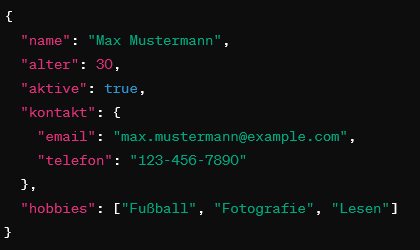
\includegraphics[width=\textwidth]{figures/jsonexample.png}
		\caption{JSON-Daten}
		\label{fig:json}
	\end{minipage}\hfill
	\begin{minipage}{0.32\textwidth}
		\centering
		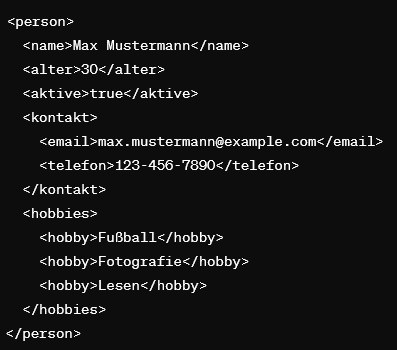
\includegraphics[width=\textwidth]{figures/xmlexample.png}
		\caption{XML-Daten}
		\label{fig:xml}
	\end{minipage}\hfill
	\begin{minipage}{0.32\textwidth}
		\centering
		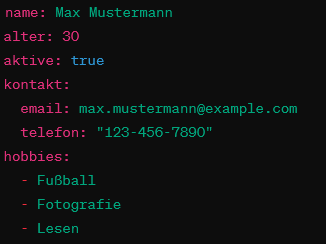
\includegraphics[width=\textwidth]{figures/ymlexample.png}
		\caption{YML-Daten}
		\label{fig:yaml}
	\end{minipage}
\end{figure}


\section{Binäre Datenformate}

Protocol Buffers (Protobuf), Cap'n Proto und Netcode for Game Objects (NfGO) sind wichtige binäre Datenformate für effiziente Datenübertragung in kritischen Anwendungsbereichen. Protobuf, von Google entwickelt, optimiert den Datenaustausch in verteilten Systemen und mobilen Anwendungen durch Codegenerierung aus .proto Dateien, bietet strikte Typsicherheit und Kompatibilität. Cap'n Proto, eine Weiterentwicklung von Protobuf, ermöglicht das Lesen von Daten ohne Umwandlung in eine Zwischenrepräsentation, wodurch die Leistung verbessert wird. NfGO, verwendet in Multiplayer-Videospielen, unterstützt synchronisierte Interaktionen durch effiziente Serialisierung und Differential Compression, um Netzwerkeffizienz und Spielerlebnis zu optimieren.

\begin{figure}[]
	\centering
	\begin{minipage}{0.48\textwidth}
		\centering
		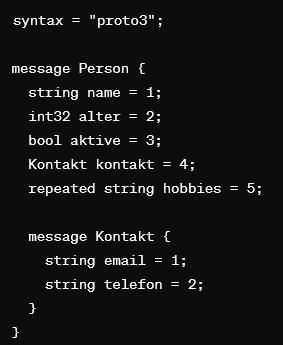
\includegraphics[width=\textwidth]{figures/protobufexample.png}
		\caption{Protobuf Datenstruktur}
		\label{fig:protobuf}
	\end{minipage}\hfill
	\begin{minipage}{0.48\textwidth}
		\centering
		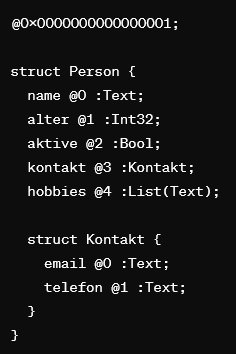
\includegraphics[width=\textwidth]{figures/capnprotoexample.png}
		\caption{Cap'n Proto Datenstruktur}
		\label{fig:capnproto}
	\end{minipage}\hfill
	
\end{figure}


\section{Serialisierung in Unity}

Unity bietet eine Reihe an Möglichkeiten an, mit denen Entwickler ihre Daten serialisieren können. Diese Methoden sind jedoch zu einem nicht unerheblichen Teil vollständig in das Unity-Universum integriert und können daher nicht außerhalb verwendet werden. Insgesamt sind für beide Projekte also einige Basiskonzepte vorhanden, die in beiden Projekten verwendet wurden.

\subsection{Byte-Arrays}

Ganz allgemein haben wir uns bei der Definition der Interfaces für die verschiedenen Aufgabenabschnitte darauf geeinigt, dass Objekte in Byte-Arrays zu serialisieren sind. Diese Byte-Arrays werden dann von der Netzwerkschnittstelle übertragen. Aus diesem Grund zielt die Umsetzung in beiden Projekten darauf ab, C\#-Klassen in Byte-Arrays zu übersetzen und zurück.

\chapter{Bibliotheken und Assets}

\section{Into the Sky}

Aufgrund der geringeren Datenmenge ist es bei performancekritischen Spielen, wie MMOFPS-Spielen, empfehlenswert, ein Binärformat zur Serialisierung von Datenstrukturen zu verwenden. Für Into the Sky habe ich michdaher für die Verwendung von Protobuf entschieden.

Im Vergleich zu neueren Verfahren wie Cap'n Proto ist deutlich mehr Dokumentation vorhanden, was die Arbeit an dem Projekt beschleunigt. Im Gegensatz zu Formaten wie JSON ist Protobuf im Hinblick auf die Datenpakete deutlich effizienter. Die Verwendung eines kompakten Binärformats verringert die zu übertragene Datenmenge erheblich. Der Nachteil von Strukturierten Formaten wie JSON ist, dass Daten wie Feldnamen oder Klassennamen mit übertragen werden. Das macht die Daten zwar leichter wartbar, in diesem Kontext ist allerdings die Effizienz von höchster Prioriät.

In der Präsentation habe ich ursprünglich vorgeschlagen Netcode for Game Objects zu verwenden. Diese Bibliothek ist jedoch nicht mit den Architekturvorschlägen und den ersten Umsetzungen kompatibel. Der Ansatz, der zu Beginn der Implementierung vorgelegen hat, basiert auf Reflection. Protobuf ist als etabliertes Verfahren jedoch vorzuziehen und bietet diverse Optimierungen, die durch einen Eigenbau nicht erreicht werden können.

\subsection{Entwicklung des Proof-of-Concept}

Der Setup-Prozess von Protobuf in Unity war erstaunlich einfach. Neben diversen Online-Turorials waren auch die Fehlerbehebungsstrategien von ChatGPT 4 sehr nützlich.

Der Prozess, um ein Proof-Of-Concept zu realisieren, ist einfach und geradlining. Als erstes wird ein  neues Projekt in Visual Studio angelegt. Dabei handelt es sich um eine "Class Library". Der Unity-Version ist zu entnehmen, dass die Objekte den .NET Standard 2.1 unterstützen. Über NuGet wird Protobuf installiert, dabei ist die aktuellste Version benutzbar (zum aktuellen Zeitpunkt 3.26.1). Anschließend wird die Struktur der Netzwerkbibliothek angelegt.

\begin{figure}[!h]
	\centering
	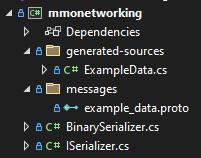
\includegraphics[width=6cm]{figures/networkingstructure.png}
	\caption{Struktur der Netzwerkbibliothek}
	\label{fig:networkingstructure}
\end{figure}

Der Ordner \verb|generated-sources| wird zunächst leer gelassen. Dort landen die ganzen generierten Dateien von Protobuf. Um die Dateien zu erstellen muss zunächst \verb|protoc| installiert werden. Anschließend muss das Bauen der Protobuf Dateien in den Build-Prozess von Visual Studio eingebunden werden. Dies geschieht, indem man den folgenden Befehl als Build-Event einfügt:

\begin{quote}
	\centering
	protoc -I="\$(ProjectDir)messages" --csharp\_out="\$(ProjectDir)generated-sources" "\$(ProjectDir)messages\*.proto"
\end{quote}

\begin{figure}[!h]
	\centering
	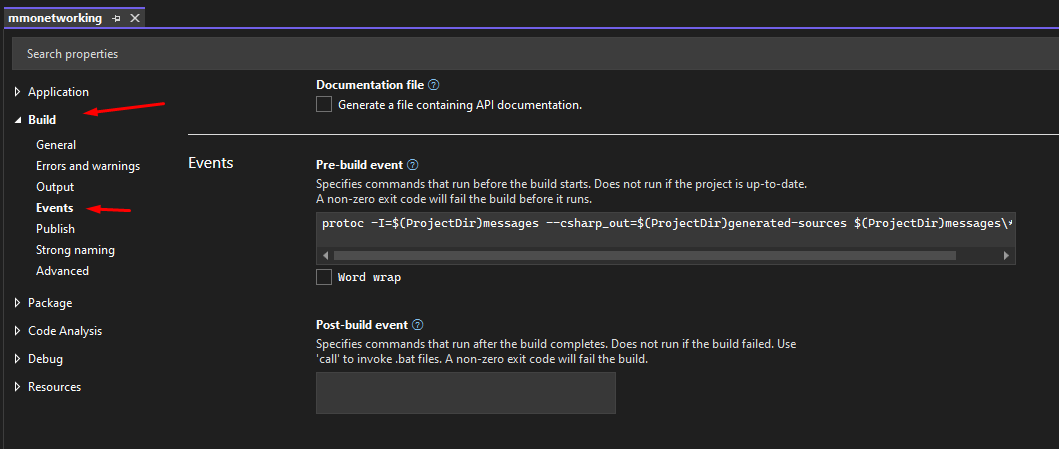
\includegraphics[width=16cm]{figures/networkingprotobuild.png}
	\caption{Build-Befehl}
	\label{fig:networkingbuildcommand}
\end{figure}

Dieser Befehl kompiliert die Proto-Dateien im messages Ordner und erzeugt die C\# Quelldateien im generated-sources Ordner. Durch das Build-Event wird dies vor jedem Kompilierprozess durchgeführt.

Nach dem Erstellen einer Muster-Datei zur Datenübertragung die einige Beispielfelder enthält wird diese zu einer C\#-Datei kompiliert. Nun kann ein einfacher Serializer geschrieben werden, der die von Protobuf bereitgestellten Methoden nutzt. Im Anschluss kann das Projekt mit \verb|Build -> Build Solution| gebaut werden. Im Output ist nun erkennbar wo sich die gebaute DLL befindet. Neben dieser DLL müssen die DLL's von Protobuf und einer Abhängigkeit von Protobuf (System.Runtime.CompilerServices.Unsafe) heruntergeladen oder aus dem System entnommen werden. Dabei wird die Version 6.0.0 der Abhängigkeit benötigt.

Diese Abhängigkeiten werden im Client-Projekt des IntoTheSky eingefügt. Der Zielordner ist \verb|Assets/Plugins|. Dorthin werden die insgesamt drei DLL's Kopiert. Diese werden dann von Unity (hoffentlich fehlerfrei) geladen.

Der PoC wird durch das Erstellen eines neuen Scripts abgeschlossen. Dort kann nun der Serializer benutzt werden. Auch die Klassen, die durch den Protobuf-Compiler erstellt wurden sind verfügbar und können zur Serialisierung der Daten benutzt werden.


\subsection{Tests}

Um die Serialisierung zu testen, habe ich ein zweites Projekt der Solution hinzugefügt. Dieses wird als \verb|MSTest Test Project| erstellt und bringt die nötigen Mittel mit, um eine Class Library zu testen. Nachdem die Class Library als Abhängigkeit eingetragen wurde kann man nun Unit-Test-Klassen schreiben. In diesem Fall habe ich folgende Testfälle initial angelegt, diese werden vermutlich im Laufe des Projekts erweitert. Die Tests werden nach einer stets gleichen Struktur benannt: Zuerst wird die Situation beschrieben, anschließend die Eingabe die getestet werden soll und zuletzt das zu erwarte

\begin{figure}[!h]
	\centering
	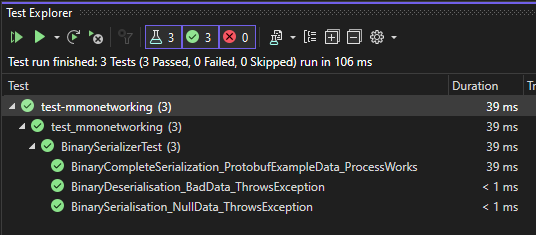
\includegraphics[width=16cm]{figures/intotheskytests.png}
	\caption{Beispielhafte Test-Cases (Into The Sky)}
	\label{fig:networkingstructure}
\end{figure}

\section{Park Chase}

Für ParkChase habe ich mich für einen einfachen JSON-Serialiser entschieden. Übertragungsgeschwindigkeit und Delay sind aufgrund des Spielkonzepts von Park Chase weniger kritisch . Außerdem wird das Spiel auf verschiedensten mobilen Endgeräten gespielt werden. Um dort vergleichsweise einfach das Spiel zu testen ist es wichtig Menschenlesbare Formate zu benutzen. In diesem Fall habe ich mich für JSON aufgrund seiner einfachen Struktur und guten Unterstützung durch Unity entschieden.

\subsection{Entwicklung der Serialisierungs-Klasse}

Unity enthält bereits eine Klasse, die die JSON Serialisierung durchführt. Dabei handelt es sich um die Klasse \verb|JsonUtility|. Die eigene Klasse beinhaltet im wesentlichen nur Aufrufe der Methoden dieser Klasse und dem Umwandeln des JSON-Strings in ein UTF-8 kodiertes Byte-Array.

\subsection{Tests}

Die Testfälle zu dieser Klasse sind ähnlich zu dem der Tests von Into The Sky aufgebaut. Hier werden allerdings die Test-Strukturen von Unity direkt verwendet. 

\begin{figure}[!h]
	\centering
	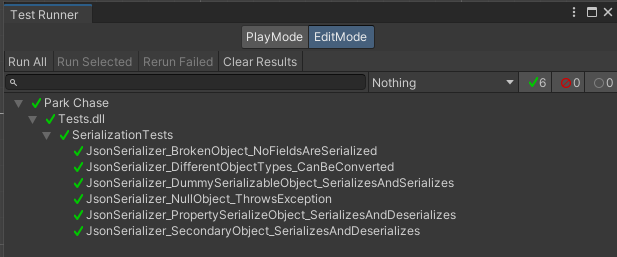
\includegraphics[width=16cm]{figures/parkchasetests.png}
	\caption{Beispielhafte Test-Cases (Park Chase)}
	\label{fig:parkchasetests}
\end{figure}

Die Test-Strukturen erlauben es auch, Tests im laufenden Spielbetrieb laufen zu lassen. Dies ist für diese Klasse jedoch nicht sinnhaft, weshalb ein Unit-Test vollkommen ausreichend ist.

\newpage



% remove if not needed
\appendix

\bibliographystyle{wmaainf}
\bibliography{refs}

\printnoidxglossaries

\end{document}
